\chapter{Ideation}
\label{Ideation}
The very first ideation session was very far from the prototype that we ended up with. It started out as a classic brainstorm and ended up revolving around making a multi-purpose Near Field Communication (NFC) RFID device which would be able to toggle the correct signal on or off depending on where it should be used. This way it would be possible to have all your RFID purposes built in to one single device such as your credit card, Rejsekortet, your access card for the university etc. This would eliminate the need for fumbling around your wallet for the correct card of which there are many these days and perhaps even making it wearable eg. a ring on one's finger or embedded in one's jacket. However, the idea did not make it very far from the drawing board after a conversation with Markus Löchtefeld who had personal experience working with this technology. It was not deemed possible. We went back to idea creation and decided to make something fun. The idea of making something wearable carried over and eventually we settled on \textit{FingerDrums}, and idea that will make it possible to drum on any surface and then have a real drum sound play. 

\section{Sketching}
The first sketches of the \textit{FingerDrums} concept is seen in \autoref{fig:sketch_1} and \autoref{fig:sketch_2}. The idea was to attach a sensor at the fingertips to register the drumming and signal the drum sound. At this point no 
\begin{figure}
\centering
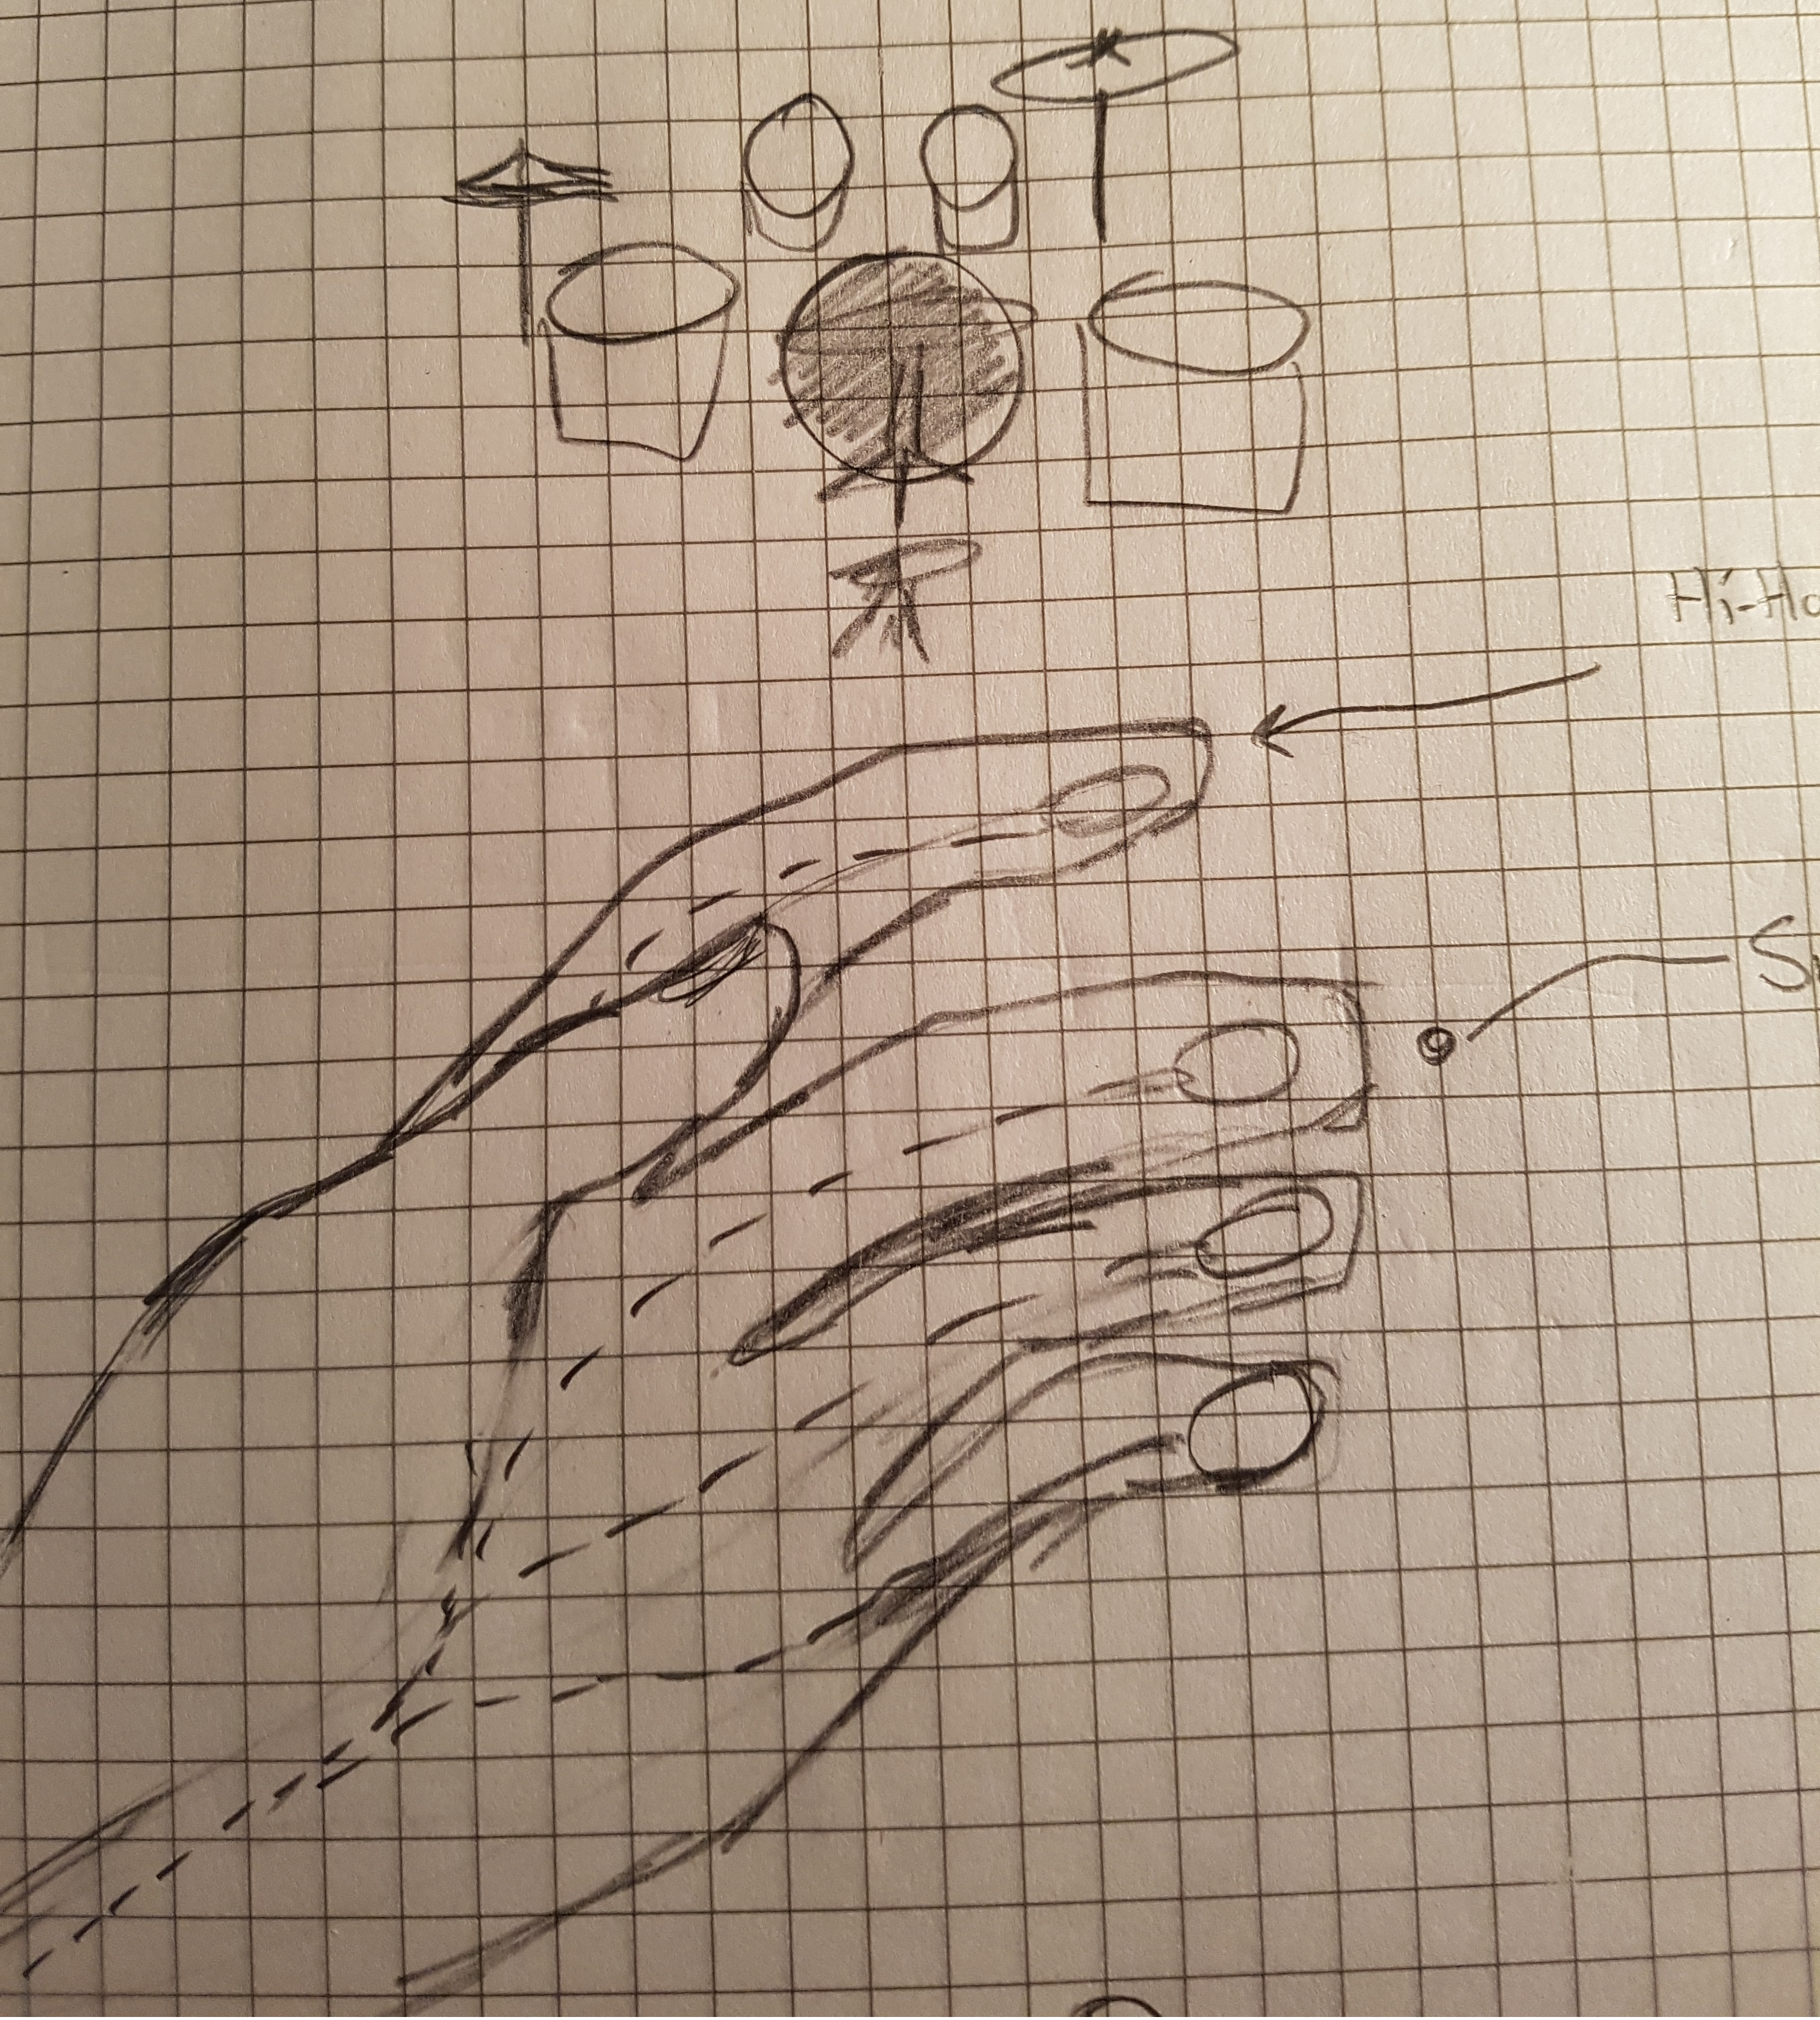
\includegraphics[scale=0.10]{Figure/sketch_1.jpg}
\caption{The first sketch of the idea to attach FSR to the finger tips as a way of drumming on any surface while still sounding like a drumkit.}
\label{fig:sketch_1}
\end{figure}



\begin{figure}
\centering
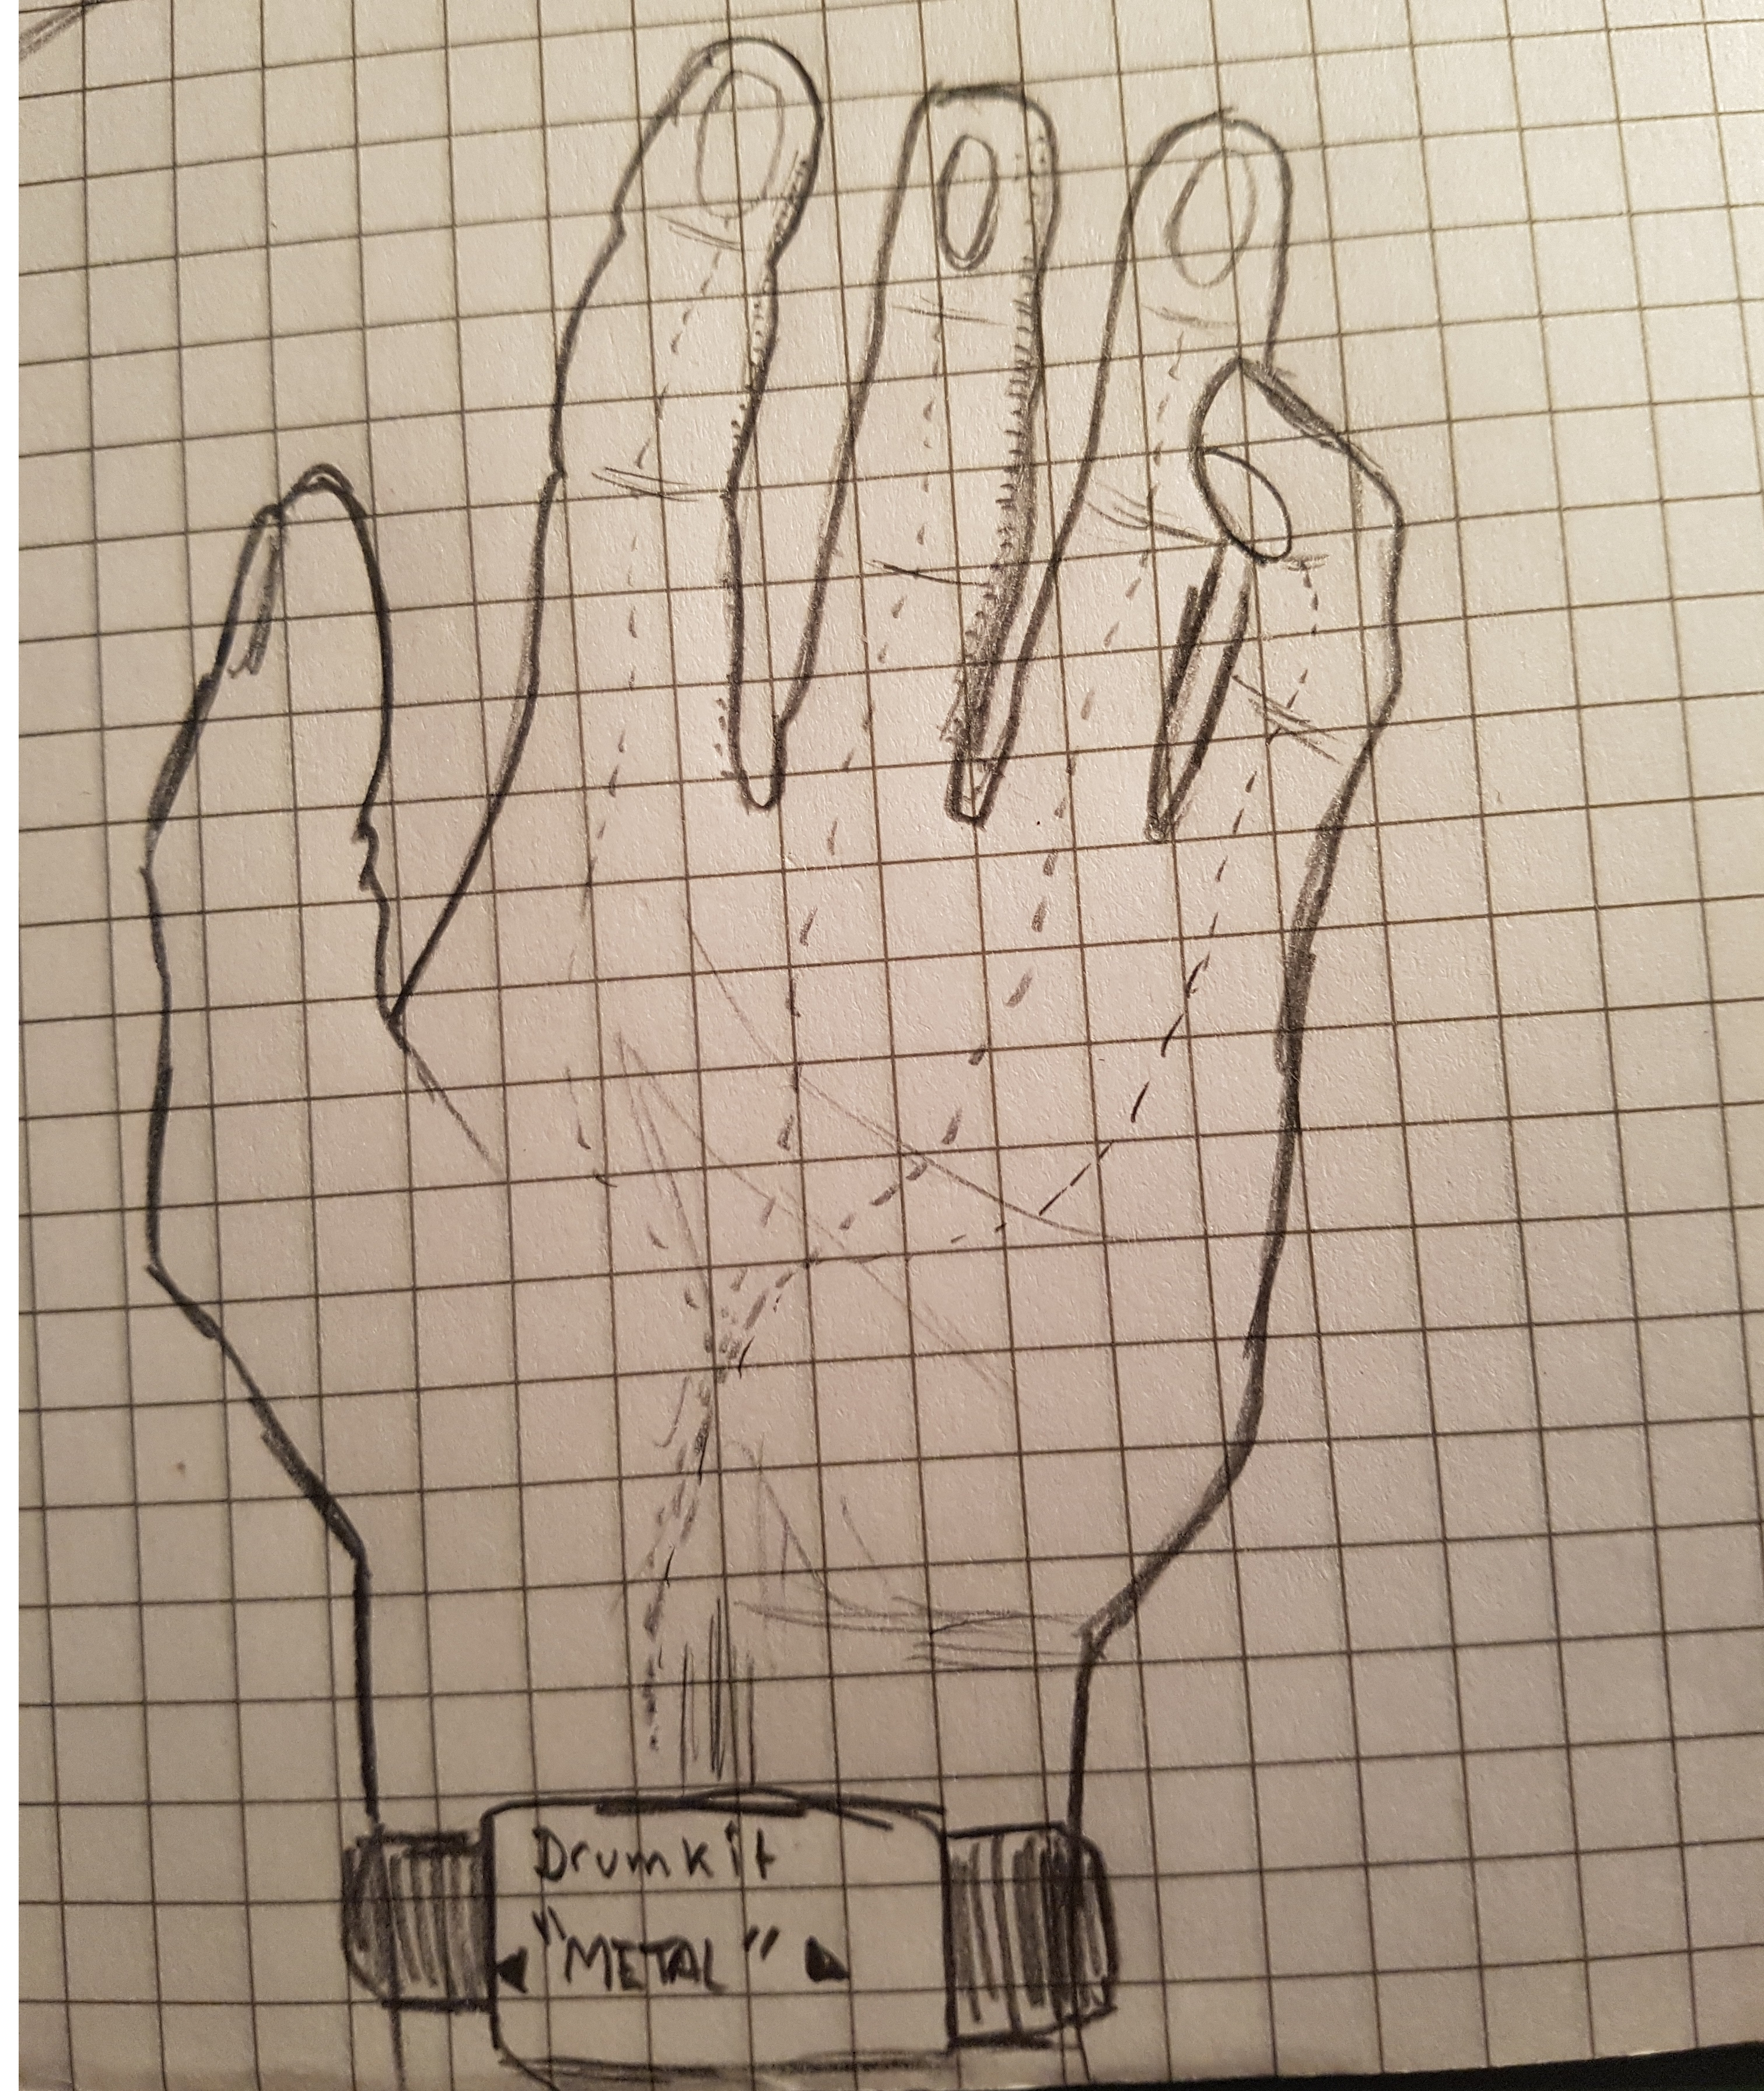
\includegraphics[scale=0.10]{Figure/sketch_2.jpg}
\caption{The second sketch of the idea to attach FSR to the finger tips as a way of drumming on any surface while still sounding like a drumkit. A small OLED display has been added in this version as a way for the user to rapid change the drum sounds if needed and a form of feedback so that the user knows what sound profile is chosen.}
\label{fig:sketch_2}
\end{figure}